\chapter{Giovedì 07/05/2020}
Le transazioni possono essere di una certa dimensione e richiedere un certo tempo per essere completate. Dobbiamo essere in grado di gestire le anomalie derivanti dall'esecuzione concorrente. Lavorare con una sola CPU significa adottare l'approccio dell'esecuzione di pezzi di transazioni alternati: questo può provocare problemi soprattutto se le due transazioni agiscono sugli stessi elementi. Segue la necessità di governare la situazione.

\section{Gestore della concorrenza}
\begin{center}
	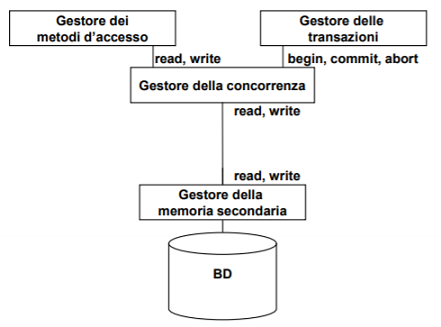
\includegraphics{images/152.PNG}
\end{center}
Il gestore della concorrenza si occupa di una parte estremamente complicata: sono necessari algoritmi estremamente sofisticati e complicati. Le transazioni devono andare avanti il più possibile. 
\subsection{Esempi di problemi}
\paragraph{Perdita di aggiornamento (W-W)} 
Utilizziamo le seguenti transazioni, identiche
\begin{itemize}
	\item $t1: r(x), x = x+1, w(x)$
	\item $t2: r(x), x = x+1, w(x)$
\end{itemize}
Inizialmente ho $x=2$, dopo un'esecuzione seriale $x=4$. In caso di esecuzioni concorrenti gestite in modo interfogliato viene perso un aggiornamento: otteniamo $x=3$.
\begin{center}
	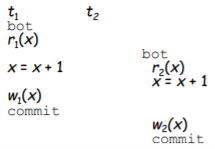
\includegraphics{images/153.PNG}
\end{center}
Nel modo indicato nell'immagine la lettura di $x$ presente nella seconda transazione non è aggiornata. Pur avendo fatto commit nella prima transazione il risultato viene sovrascritto: il risultato della seconda transazione, posto dopo quello della prima, si basa su una lettura non aggiornata.
\begin{multicols}{2}
	\paragraph{Lettura sporca (R-W o W-W con abort)} La prima transazione viene abortita, tuttavia la seconda ha letto risultati intermedi della prima: con questo si intende il valore di $x$ incrementato prima dell'abort (con l'abort l'operazione viene annullata).
	\begin{center}
		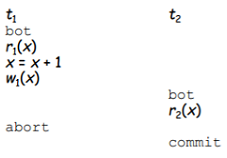
\includegraphics{images/154.PNG}
	\end{center}
	\paragraph{Lettura inconsistenti (R-W)} Nella prima transazione si svolgono due operazioni di lettura di $x$. Nell'esempio qua sotto il primo $x$ dipende dallo stato iniziale della base di dati, il secondo dipende dalla seconda transazione. Segue la lettura di due valori $x$ diversi! 
	\begin{center}
		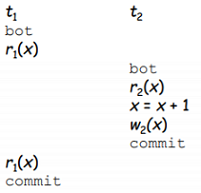
\includegraphics{images/155.PNG}
	\end{center}
	Si individuano letture diverse anche nei seguenti casi: entrambe le operazioni di lettura svolte prima del \emph{bot} della seconda transazione; entrambe le operazioni di lettura svolte dopo il \emph{commit} della seconda transazione.
\end{multicols}
\paragraph{Aggiornamento fantasma (R-W)} Assumiamo ci sia un vincolo $y+z=1000$. La prima transazione $y$ e $z$. Il primo dipende dallo dato iniziale del db, il secondo dipende dalla seconda transazione. 
\begin{center}
	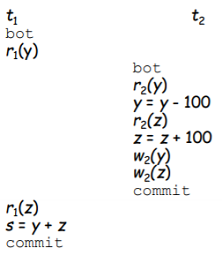
\includegraphics{images/156.PNG}
\end{center}
Segue che $y$ potrebbe dare problemi. Osserviamo che al termine della prima transazione, dopo aver sommato $y$ e $z$,si ha come risultato $1100$: ciò viola il vincolo stabilito.

\paragraph{Inserimento fantasma (R-W)} Cosa analoga: prima leggo gli stipendi degli impiegati nella prima transazione e dopo, nella seconda transazione, inserisco un nuovo dipendente.
\begin{center}
	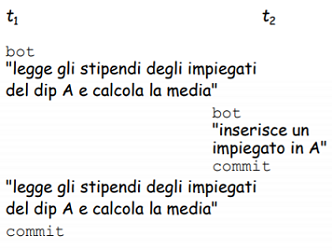
\includegraphics{images/157.PNG}
\end{center}

\subsubsection{Ricapitoliamo}
\begin{itemize}
	\item \textbf{Perdita di aggiornamento (W-W)}: Abbiamo due transazioni che effettuano operazioni di scrittura su un oggetto. Le operazioni si basano su una precedente lettura. Il problema è che una delle letture non legge il dato aggiornato: segue che una delle due modifiche risulta persa!
	\item \textbf{Lettura sporca (R-W o W-W con abort)}: ho una transazione che legge e scrive e una che legge. La prima transazione abortisce, ma la seconda nel frattempo ha letto il valore di $x$ modificato.
	\item \textbf{Letture inconsistenti (R-W)}: ho una transazione che svolge due operazioni di lettura e una che svolge un'operazione di lettura seguita da una di scrittura. In uno schedule serializzabile non è possibile che le due operazioni di lettura restituiscano valori diversi!
	\item \textbf{Aggiornamento fantasma (R-W)}: Abbiamo una transazione che legge dei valori aggiornati da un'altra transazione. L'interleaving potrebbe portare alla violazione di vincoli precedentemente imposti.
	\item \textbf{Inserimento fantasma (R-W)}: una transazione potrebbe effettuare una lettura di una serie di valori e successivamente usarli per calcolare un risultato. Tra la prima e la seconda cosa si ha l'inserimento, da parte di una seconda transazione, di un nuovo valore: questo sarà ignorato.
\end{itemize}

\subsection{Come gestire?} 

\paragraph{Schedule} Dato che più transazioni vengono eseguite in modo concorrente le operazioni di scrittura/lettura vengono richieste da transazioni differenti in interleaving. Uno schedule consiste in una sequenza di operazioni di lettura/scrittura relativa a un insieme di transazioni concorrenti. Per fare ciò eseguiamo operazioni di \emph{scheduling}, operazione fondamentale del controllore della concorrenza. Fondamentalmente: 
\begin{itemize}
	\item elenco delle operazioni di lettura e scrittura applicate ad oggetti; 
	\item se la sequenza è permessa si ha come risultato finale un qualcosa ottenibile anche attraverso un'esecuzione in sequenza di istruzioni.
\end{itemize}

\paragraph{Controllo di concorrenza} Il gestore, per evitare anomalie, determina un ordine delle richieste fatte. Continua ad accettare gli ordini finchè non si rende conto che accettando una certa operazione si avrebbe un qualcosa di assolutamente incompatibile con un comportamento seriale. Questa richiesta viene fermata e messa da parte finchè l'oggetto incriminato nell'operazione non sarà "liberato".\\

\noindent Tutte le sequenze di operazioni che risultano completate rappresentano degli schedule serializzabili, cioè equivalenti a qualche schedule seriale. Il comportamento seriale è corretto per definizione e non può portare problemi.

\paragraph{Idea di base} L'obiettivo è individuare classi di schedule serializzabili la cui proprietà di serializzabilità sia verificabile a costo basso (tenendo conto che le operazioni vengono fatte online). 
Cioè, come posso capire se quell'esecuzione (con operazioni in un certo ordine) ci porterà a ottenere un qualcosa di serializzabile?
\begin{center}
	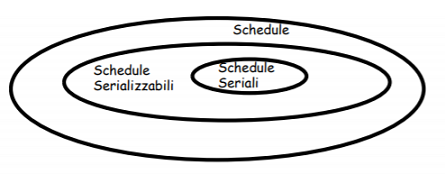
\includegraphics{images/158.PNG}
\end{center}

Distinguo schedule seriali da schedule serializzabili e infine schedule non serializzabili. Tutto ciò che è stato fatto deve essere buttato via se non è possibile ottenere un qualcosa di serializzabile. Attraverso algoritmi devono individuare classi di schedule grandi: più grandi saranno, migliore potrà essere considerato l'algoritmo.